\begin{newpage}
	\section{Einleitung}
	\label{sec:Einleitung}
	 %  Data can be rather complex. To understand complex systems we have different approaches in our professions. In software development we have tools like "Divide and Conquer" to help us break things into smaller pieces. But what if that does not help us understanding the fundamental underlying principles. Bret Victor describes in his essay "Up and Down the Ladder of Abstraction" a more visual approach for finding a profound insight into complex systems: 

	 %  \begin{quote}
		% 	\emph{"`When designing [a system], the challenge lies not in constructing the system, but in understanding it. In the absence of theory, we must develop an intuition to guide our decisions. The design process is thus one of exploration and discovery."'} \parencite{victor}
		% \end{quote}

	 %  Data is often coupled to each other. Separating it into smaller junks can alter its meaning, because the context could get lost or changed. Often times interesting datasets are described interesting especially because they have relations that tell a story. Thats why data visualization got so popular in this decade. We searched for new exciting ways of exploring data and tell untold stories. Especially on maps we are seeing all kinds of neat visualizations, giving data a geospatial context. Ranging from demographic health coverage, crime rates, earthquake data for different regions to a live aircraft flight radar.

		% Visualizations help us to understand complex topics in a more consumable way. They enable us to explore data, exposing twists and secrets that otherwise might have been left buried in that huge pile that data often times is.\\

		Datenvisualisierung ist ein Thema, das nicht nur in jüngster Zeit sehr viel Zuwendung fand, sondern auch zur Analyse von Sachverhalten immer wichtiger wird. So lassen sich komplexe Zusammenhänge eines Systems, oftmals erst dann richtig begreifen, wenn wir alle möglichen Zustände davon erfassen können. In "`Up and Down the Ladder of Abstraction"', beschreibt Bret Victor wie sich Systeme in ihrer Ganzheit besser begreifen und gestalten lassen.

		\begin{quote}
			\emph{"`When designing [a system], the challenge lies not in constructing the system, but in understanding it. In the absence of theory, we must develop an intuition to guide our decisions. The design process is thus one of exploration and discovery."'} \parencite{victor}
		\end{quote}

		Auch eine Ansammlung an Daten ist erst einmal sehr abstrakt. In einer Datenbank in Relation gebracht, bleiben die meisten Erkenntnisse und Stories verborgen. Ein tieferes Verständnis, begreifen wir erst dann, wenn wir sie auswerten. Die Art der Datenvisualisierung hat sich in den letzten Jahren stark gewandelt. Während anfangs vor allem Daten in der Form von Häufigkeitsanalysen ausgewertet und als Bar- oder Linechart visualisiert wurden, haben wir heute interaktive Karten um raumbezogene Zusammenhänge zu veranschaulichen.

		Diesen Trend von dynamischen Live Visualisierungen findet in verschiedensten Bereichen Einzug. Zum Beispiel der erst kürzlich erschienene Flight-Planner des Dubai Airports\footnote{\url{http://www.dubaiairports.ae/flight-planner}}, die Marine-Traffic-Map\footnote{\url{https://www.marinetraffic.com/}} in der Schifffahrt oder auch für die Live Simulation von Wetterdaten\footnote{\url{https://www.windy.com/}}. 

		Auch regional gibt es verschiedene Produkte die veröffentlicht wurden. Beispielsweise der Zugradar\footnote{\url{http://bahn.de/zugradar}} (2014) und der Busradar\footnote{\url{https://play.google.com/store/apps/details?id=de.hafas.android.dbbusradar}} der Deutschen Bahn oder eine Karte für das S-Bahn Netz in München\footnote{\url{http://s-bahn-muenchen.hafas.de/}} (2009).

		Eine gesamte Erfassung des öffentlichen Verkehrs ging ebenfalls 2014 mit Travic\footnote{\url{http://tracker.geops.de/}}\label{travic} online und bietet mit über 650 integrierten Fahrplänen eine enorme Abdeckung. Da die Live Karten der Deutschen Bahn damals nur die Visualisierung der eigenen Bus und Bahnlinien ermöglichte, war Travic darin bestrebt diese Lücke zu schließen und den gesamten öffentlichen Verkehr darzustellen. 
		Zusätzlich sei noch LiveMap24 \footnote{\url{https://www.livemap24.com/}} von Verdict erwähnt. Auch eine Live Karte, deren Veröffentlichungsdatum mir allerdings nicht bekannt ist.

		Der Vorteil einer Digitalen Karte besteht in seiner ständigen Aktualität. Ein statischer Fahrplan kann keine Informationen zu Störungen, Verspätungen oder Ausfall eines Zuges geben. Auf einer Live Karte lassen sich solche Informationen visuell aufbereiten und dem Anwender über die Benutzeroberfläche vermitteln. Der Betrachter kann sehen wie viele Fahrzeuge gerade aktiv sind und kann zusätzlich zum statischen Fahrplan auch visuell erleben wo sich sein Zug oder Bus befindet. 
		Da gleichzeitig Fahrplan als auch Karte vorhanden sind, ist auch eine geographische Orientierung möglich. \emph{"`Der Zug hat 5 Minuten Verspätung"'} wird ein visueller Kontext gegeben und ist dadurch nicht mehr nur eine Aussage, sondern erfahrbar.
    Einen Nutzen in einer Live Karte sehen aber nicht nur Pendler oder Reisende, sondern auch Verkehrsunternehmen, Städte oder Verkehrsforscher.\\
		
		%Durch die erstell... lassen sich Erkenntnisse gewinnen, die durch diese Form der Visualisierung Einblicke ermöglichen, die durch eine gedruckte 2D Karte in dieser Art, nicht möglich gewesen währen.\\

		Diese Arbeit befasst sich umfassend mit der Entwicklung einer Live Karte für den öffentlichen Nahverkehr anhand von GTFS Daten. Der Fokus liegt dabei in der Gestaltung von verschiedenen Visualisierungen, welche die User Experience erhöhen und die Karte nicht nur interaktiv, sondern vor allem auch dem Benutzer Freude bei der Bedienung bereitet.

		\subsection{The Double Diamond}
\label{sub:the_double_diamond}
  Das Projekt wurde nach dem Design Prozess \texttt{"`The Double Diamond"'}\footnote{\url{http://www.designcouncil.org.uk/news-opinion/design-process-what-double-diamond}} bearbeitet. Der Double Diamond wurde vom British Design Council 2005 entwickelt und soll im folgenden danach beschrieben werden.\parencite{designcouncil}

  \begin{figure}[htbp]
    \begin{center}
      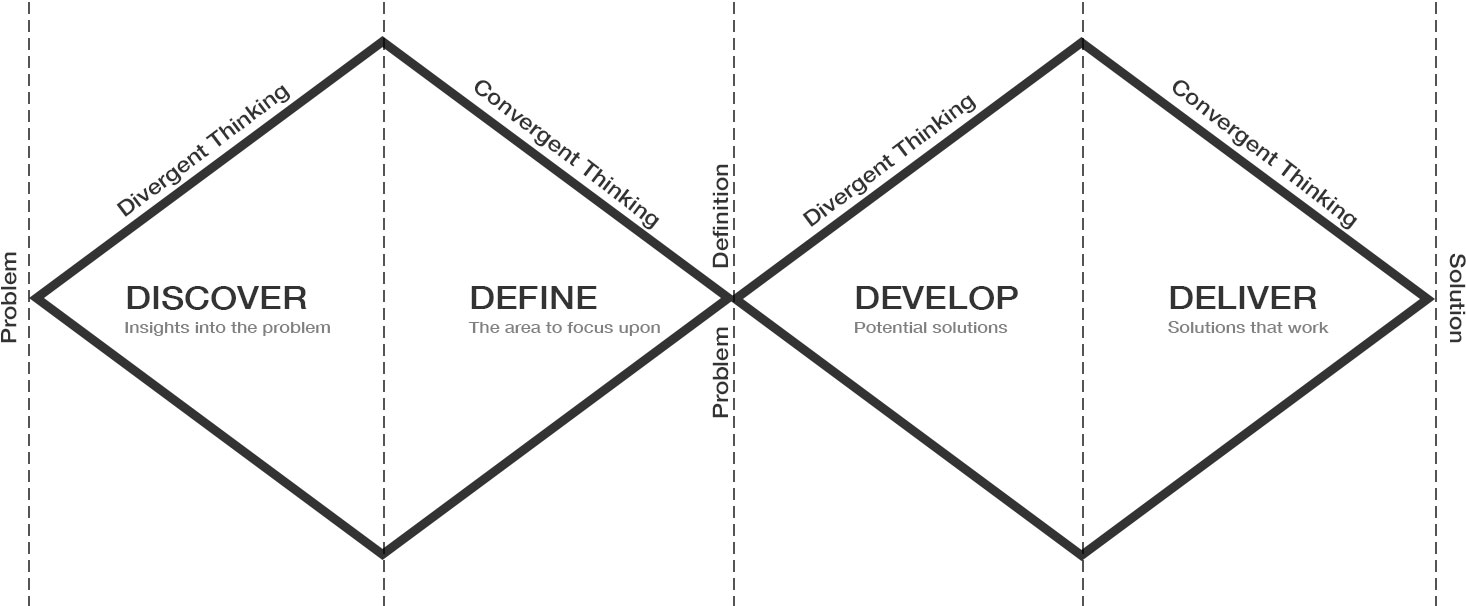
\includegraphics[width=0.9\textwidth]{double_diamond}
      \caption{"`The Double Diamond"' eigene Abbildung nach \parencite{designcouncil}}
      \label{fig:double_diamond}
    \end{center}
  \end{figure}

  Der Double Diamond beschreibt ein iterative Prozess. Wie in allen kreativen Prozessen werden dabei eine Reihe von möglichen Ideen geschaffen ("divergentes Denken"), bevor sie verfeinert und auf die beste Idee reduziert werden ("konvergentes Denken"). Der Double Diamond zeigt jedoch an, dass dies zweimal geschieht - einmal zur Bestätigung der Problemdefinition und einmal zur Erstellung der Lösung. Einer der größten Fehler ist es, den linken Diamanten wegzulassen und am Ende das falsche Problem zu lösen.

  \begin{itemize}[label={}]
    \item \textbf{Discover:} Der erste Teil des Double Diamond steht am Anfang des Projektes. Hier wird versucht, die Welt neu zu sehen, Neues wahrzunehmen und Einsichten in das zu lösende Problem zu sammeln.

    \item \textbf{Define:} Der zweite Teil stellt die Definitionsphase dar. Dabei wird versucht alle in der Entdeckungsphase identifizierten Möglichkeiten zu verstehen. Ziel ist es dabei, ein klares Briefing zu entwickeln, das die grundsätzlichen Herausforderungen umrahmt.

    \item \textbf{Develop:} Der dritte Teil markiert eine Entwicklungsphase, in der Lösungen oder Konzepte erstellt, prototypisiert, getestet und iteriert werden. Dieser Prozess des Ausprobierens hilft, Ideen zu verbessern und zu verfeinern.

    \item \textbf{Deliver:} Der letzte Teil des Double Diamond ist die Lieferphase, in der das daraus resultierende Projekt (z. B. ein Produkt, eine Dienstleistung oder eine Umwelt) abgeschlossen, produziert und in Betrieb genommen wird.
  \end{itemize}

% sub:the_double_diamond (end)

		% Aufzählen der eigenen Features der Karte. Was für Sachen wurden entworfen etc.

		% Aufzählen was in den einzelnen Kapiteln noch alles behandelt wird.

\end{newpage}